\documentclass{article} % For LaTeX2e
\usepackage{nips15submit_e,times}
\usepackage{hyperref}
\usepackage{url}
\usepackage{amsmath}
\usepackage{graphicx}
\usepackage{placeins}
\usepackage{multicol, multirow, array}

\newcommand{\mc}[2]{\multicolumn{#1}{#2}}

%\documentstyle[nips14submit_09,times,art10]{article} % For LaTeX 2.09

\title{A Comparative Study of Matrix Completion Methods}

\author{
Sriram Ganesan\thanks{ The names are printed in alphabetical order by last name.} \\
\texttt{sriramg@umich.edu} \\
\And
Nitin Garg \\
\texttt{gargn@umich.edu} \\
\AND
Jeeheh Oh \\
\texttt{jeeheh@umich.edu} \\
\And
Jonathan Stroud \\
\texttt{stroud@umich.edu} \\
}

\newcommand{\fix}{\marginpar{FIX}}
\newcommand{\new}{\marginpar{NEW}}

\nipsfinalcopy % Uncomment for camera-ready version

\begin{document}

\maketitle

\begin{abstract}
Matrix completion, is the task of filling in the unknown entries of a sparse matrix. This problem is central in recommender systems and collaborative filtering, which provide individualized product suggestions based on ratings gathered from a large set of users. Matrix completion algorithms are used effectively today to provide helpful recommendations for users of services such as Netflix and Amazon.com. In the present paper, the baseline algorithms for matrix completion, such as eigentaste, nearest K-neighbor, and column mean are compared against the more sophisticated matrix completion algorithms, such as Spectral Matrix Completion (SMC) and Singular Value Thresholding (SVT). The comparison metric used in the present paper include, accuracy, convergence time, and the nature of the input matrix. All of the presented methods have their advantages and disadvantages based on the problem. In the present paper, the detailed results are presented for synthetic data and the Jester data. While Eigentaste needs at least few fully filled columns to complete the sparse matrix, SMC and SVT does not have that limitation. Between SMC and SVT, SMC provides better accuracy but is much slower than the SVT. Detailed comparison of the methods is presented in the later sections.

\end{abstract}

\section{Introduction}

How can we predict what movies a person will enjoy? On what web-pages
will they click? Which emails will they read? \emph{Collaborative
  Filtering} problems like these are tricky. Consider predicting a
person's movie preferences using Netflix's database. We can predict
how highly a user will rate the movie \textit{Rambo} using a
regression model trained on the ratings of users that have rated
\textit{Rambo} before. We quickly run into problems when we realize
that most users have not rated \textit{Rambo}, and most users who
have, have not rated the same ones as the user for whom we are making
the prediction. This means that our model would have to ignore a
majority of the data available, limiting performance. Furthermore a
separate model would need to be trained for each movie in the system,
leading to computational difficulties.

A better framework for these sorts of problem is \emph{matrix
  completion}. We can view each user-item pair as an entry in a matrix
that has only a few entries filled in. Our task is then to complete
the matrix, assuming that it has some simple underlying structure. Low
rank is a common structural assumption. Recovering a low rank matrix
from a few entries is a problem with applications not only in
collaborative filtering~\cite{r25}, but also in dimensionality
reduction~\cite{r20, r28} and multi-task learning~\cite{r2, r22}. This
problem turns out to be computationally hard. In fact, rank
minimization is NP-hard, meaning that is at least as hard as all those
that can be solved by a nondeterministic Turing machine in polynomial
time, like the Hamiltonian Cycle~\cite{plesn} and Traveling Salesman problems~\cite{lawler1985}. In
both theory and practice, all algorithms that perform this task have
time complexity exponential in the size of the matrix.

Candes and Recht showed that most low-rank matrices could be recovered instead by minimizing the nuclear norm, defined as the sum of the
singular values~\cite{r4}. Theoretically, the nuclear
norm is the tightest convex lower bound on the rank function for
singular values no greater than 1. Intuitively, while the rank
function counts the number of nonzero singular values, the nuclear
norm sums their amplitude, much like how the 1-norm is a useful
substitute for counting the number of nonzero entries in a vector.
Conveniently, the nuclear norm can be minimized efficiently subject to
equality constraints via semidefinite programming.

Nuclear norm minimization has long been observed to produce fairly
low-rank solutions~\cite{r11, r12, r26}, but only recently there was
any theoretical basis for the instances where it produced the true
minimum rank solution. One of the first papers to provide such
foundation was~\cite{r24}, where Recht, Fazel, and Parrilo developed
probabilistic techniques to study average case behavior. They showed
that the nuclear norm heuristic could solve most instances of the rank
minimization problem when the number of linear constraints was
sufficiently large. This inspired interest in theoretical guarantees
for rank minimization, and these results lay the foundation
for~\cite{r4}. Candes and Recht’s bounds were subsequently improved by
Candes and Tao~\cite{r7} and by Keshavan, Montanari, and
Oh~\cite{keshavan2010matrix}. They show that one could, in special
cases, reconstruct a low-rank matrix by observing a set of entries of
size at most a polylogarithmic factor larger than the intrinsic
dimension of matrix.

To test the practical validity of these theoretical guarantees, we
explore two competing algorithms for matrix completion via nuclear
norm minimization. We compare their performance on collaborative
filtering baselines, using both synthetic and real-world data. The
Singular Value Thresholding (SVT) algorithm was introduced in ``A
Singular Value Thresholding Algorithm for Matrix Completion''
\cite{cai2010singular}. Spectral Matrix Completion (SMC) was
introduced in ``Matrix Completion from a Few Entries''
\cite{keshavan2010matrix}.

\section{Singular Value Thresholding}

Formally, Singular Value Thresholding (SVT) addresses the optimization
problem
\begin{equation*}
\begin{aligned}
  & \underset{X}{\text{minimize}} & & \|X\|_{*} \\
  & \text{subject to}             & & \mathcal{P}_\Omega (X) =
  \mathcal{P}_\Omega (M), \\
\end{aligned}
\end{equation*}
where $\|\cdot\|_{*}$ is the \emph{nuclear norm}, or the sum of the
singular values, and $\mathcal{P}_\Omega (\cdot)$ is the projection
operator, which makes zero all entries $(i, j) \notin \Omega$.

Singular Value Thresholding works in an iterative, alternating fashion
reminiscent of the Alternating Direction Method of Multipliers (ADMM).
The complete matrix $X$ is constructed iteratively using a low-rank,
low-singular value approximation to an auxiliary sparse matrix $Y$.
$Y$ is then adjusted to ensure the resulting approximation in the
subsequent step has matching entries $X_{ij} = M_{ij}$. Each iteration
consists of the inductive steps
\begin{equation*}
\begin{cases}
X^{k} = \mathrm{shrink}(Y^{k-1}, \tau) \\
Y^{k} = Y^{k-1} + \delta_k \mathcal{P}_\Omega (M-X^{k}),              \\
\end{cases}
\end{equation*}
where $\mathrm{shrink}(\cdot, \cdot)$ is the \emph{singular value
  shrinkage operator}, which reduces each singular value by a given
singular value decomposition $X = U \Sigma V^T$,
$\Sigma = \mathrm{diag}(\{\sigma_i\}_{1 \le i \le r})$, we can write
this as
\begin{equation*}
\mathrm{shrink}(X, \tau) = U\Sigma_\tau V^T, \ \ \Sigma_\tau = \mathrm{diag}(\{(\sigma_i-\tau)_{+}\}).
\end{equation*}


When applied repeatedly, these steps, approach a low-nuclear norm
solution by steadily shrinking the singular values of X. This
algorithm has shown success in recovering accurate low-rank solutions
when the source of $M$ is also low-rank, even though it does not
optimize this objective directly.

SVT has hyperparameters that must be carefully tuned to guarantee
convergence. The shrinkage value $\tau$ must be set high in order for
the algorithm to converge, but not too high that it exceeds the true
singular values. The stepsizes $\delta_k$ are similarly sensitive. The
stepsize can be set dynamically or statically, though we choose to
maintain a fixed stepsize throughout. Furthermore, we compute the
decomposition of $Y^K$ in batches, which introduces a new batch size
parameter $l$ that effects the speed of convergence. Also important is
the initialization of $Y$, for which the authors provide helpful
strategies. Finally, we use the relative error
$\|\mathcal{P}_{\Omega}(X^k-M)\|_F / \|P_{\Omega} (M)\|$ as a stopping
criterion. We terminate when this drops below a small $\epsilon$.

We find from experimentation that SVT is frustratingly sensitive to
the settings of these parameters. The suggested settings only lead to
convergence for a limited range of matrix sizes and ranks, and
choosing the correct settings often requires unrealistic knowledge of
the underlying matrix structure.

\section{Spectral Matrix Completion}

Spectral Matrix Completion (SMC), presented in Keshavan et al.
\cite{keshavan2010matrix} minimizes the reconstruction error of a
low-rank matrix. Let $M$ be the complete matrix and $M^E$ be the
$m \times n$ matrix with known entries $(i,j) \in E$ filled in and
zero entries otherwise. That is,
\begin{equation}
M^E_{i,j} = \begin{cases}
    M_{i,j} & \text{if} \ \  (i,j) \in E \\
    0      & \text{otherwise}.
   \end{cases}
\end{equation}

As presented in~\cite{keshavan2010matrix}, the SMC algorithm has three
steps.
\begin{enumerate}
\item Trim $M^E$, giving $\widetilde{M}^E$.
\item Project $\widetilde{M}^E$ to $T_r(\widetilde{M}^E)$.
\item Clean, minimizing the reconstruction error $F(X,Y)$.
\end{enumerate}

\subsection{Trimming}
In the trimming step, we throw out information in order to make the
underlying true-rank structure more apparent. First, we set to zero
all columns in $M^E$ with degree larger than $2|E|/n$ and set to zero
all rows with degree larger than $2|E|/m$, where $|E|$ is the number
of non-zero entries in $M$. This step is crucially important when the
number of revealed entries per row/column follows a heavy tail
distribution, as is the case for most of the real data.

\subsection{Projection}
In the projection step, we build a low-rank reconstruction of $M^E$.
We begin by computing its the singular value decomposition (SVD). Let
the singular values be
$\sigma_1 \ge \sigma_2 \ge ... \sigma_{\min(m,n)} \ge 0$. Therefore,
the decomposition can be written as,
\begin{equation}
  M^E = \sum_{i=1}^{\min(m,n)} \sigma_ix_iy_i^T.
\end{equation}
The projection
\begin{equation}
  T_r(M^E) = \frac{mn}{|E|}\sum\limits_{i=1}^r \sigma_ix_iy_i^T
\end{equation}
is obtained by zeroing all but the $r$ largest singular values. Note
that apart from the rescaling factor $(mn/|E|)$, $T_r(M^E)$ is the
orthogonal projection of $M^E$ onto the set of rank-r matrices. The rank of the matrix, $r$, should either be supplied by the user or it will be estimated using the change in consecutive singular values.

\subsection{Cleaning}
This is the step where actual optimization takes place in SMC algorithm. We
``clean'' the errors produced by the projection step by iteratively
minimizing the reconstruction error. Given $X \in R^{m\times r}$,
$Y \in R^{n\times r}$ with $X^TX = mI$ and $Y^TY = nI$,
\begin{equation}
  F(X,Y) = \min_{S \in R^{r \times r}} F(X,Y,S)
\end{equation}
\begin{equation}
  F(X,Y,S) = \frac{1}{2} \sum\limits_{(i,j) \in E} (M_{ij} - (XSY^T)_{ij})^2
\end{equation}
We initiliaze $T_r(\widetilde{M}^E) = X_0S_0Y_0^T$ and minimize
$F(X, Y)$ locally with initial condition $X = X_0$, $Y = Y_0$. Note
that $F(X, Y)$ is easy to evaluate since it is defined by minimizing
the quadratic function $S \mapsto F(X, Y, S)$ over the low-dimensional
matrix $S$. Further, it depends on $X$ and $Y$ only through their
column spaces. In geometric terms, $F$ is a function defined over the
cartesian product of two Grassmann manifolds. Optimization over
Grassmann manifolds is a well understood
topic~\cite{edelman1998geometry} and efficient algorithms (in
particular Newton and conjugate gradient) can be applied. In our
implementation, we minimize $F(X, Y)$, using gradient descent with
line search.


\section{Baseline Algorithms}

For comparison, we introduce two simple baseline algorithms for matrix
completion.

\subsection{Eigentaste}

Eigentaste \cite{r31} is an another collaborative filtering algorithm specifically
designed for the Jester Dataset. It relies on the assumption that a
subset of the columns will be dense, corresponding to a few ``seed''
items which every user is required to review. Eigentaste applies
principal component analysis to this dense subset of columns, reducing
dimensionality and allowing rapid clustering. Recommendation is done
by averaging ratings over clusters.

Mean rating of the jth item in the gauge set is given by
\begin{equation*}
\mu_{ij}=\frac{1}{n}{\sum_{i\epsilon U_{j}}}\widetilde{r}_{ij}\\
\end{equation*}
\begin{equation*}
\sigma_j^2=\frac{1}{n-1}{\sum_{i\epsilon U_{j}}}({\widetilde{r}_{ij}-\mu_{j}})^{2}
\end{equation*}
where $\widetilde{r}_{ij}$ is the user rating of item $j$ by user $i$, $\mu_{j}$ and $\sigma_j$ is the mean and variance of the item $j$, respectively. In A, the normalized rating $r_{ij}$ is set to
$({\widetilde{r}_{ij}-\mu_{j}})/\sigma _{j}$ . The global correlation
matrix is given by
\begin{equation*}
C=\frac{1}{n-1}A^{T}A=E^{T} \Lambda E
\end{equation*}

The data is projected along the first $v$ eigenvectors
$x=R{E_{v}}^{T}$. The algorithm then proceeds as follows.

\textit{Recursive Rectangular Clustering: }

\begin{enumerate}
\item Find the minimal rectangular cell that encloses all the points
  in the eigenplane.
\item Bisect along x and y axis to form 4 rectangular sub-cells.
\item Bisect the cells in step 2 with origin as a vertex to form
  sub-cells at next hierarchical level.
\end{enumerate}

When a new user arrives, Eigentaste collects their ratings on the seed
set and projects them into the 2-dimensional eigenplane. The user is
then placed in a cluster, and recommendations are given based on the
average ratings of other users in the same cluster.

\subsection{K-Nearest Neighbors}
In the K-Nearest Neighbors algorithm, we predict ratings based on the
mean ratings of each person's nearest neighbors.
\begin{equation*}
  p_{ij}=\overline{r_{i}}+\kappa\sum_{k=1}^n w(i,p)(\overline{r_{pj}}-\overline{r_{p}})
\end{equation*}
where $\overline{r_{i}}$ is the average joke rating for user i, and
$\kappa$ is a normalizing factor ensuring that the absolute value of
the weights sum to 1. We used a function of Euclidean distance from
user $i$ to user $p$ as the weight $w(i, p)$, and $\kappa$ =
$\sum_{k=1}^n w(i,p)$. Specifically, if we are interested in $q$
nearest neighbors, $w(i; p) = d(i, q +1)- d(i, p)$. This ensures that
i’s closest neighbor have the largest weight. In our experiments, we
use a neighborhood size of $K=50$.

\section{Experimental Results}

\subsection{Synthetic Data}

We compare the performance of SVT and SMC on synthetically generated
matrices of varying ranks, sizes and sparsity. Specifically, the
algorithms were tested on all combinations of matrix size (1000,
5000), rank (5, 10 and 20), and sparsity (30\%, 50\% and 70\%). We
compare the performance of SVT and SMC, with a simple baseline, the
column mean, which predicts the average column value for all missing
entries. In Table ~\ref{Time} the mean absolute error and the run time
is averaged over the categories of size, rank, and sparsity. For
example, out of the eighteen tests that were run, nine tests include
the matrix of size 1000 $\times$ 1000. Therefore the mean absolute
error value for all nine tests are averaged in order to represent the
values in the size 1000 column of the table below. Mean absolute error
is the absolute value of the average error on the unknown entries. Run
time is measured in seconds and all simulations were run at University
of Michigan's CAEN lab computers (8GB memory with one core i7
processors). The columns in Tables 1,~\ref{Time} contain the averaged
mean absolute error and the run time for all experiments.



% I ran this experiment but the results were pretty boring. We can
% choose include them if we want (Just uncomment) but it looks like we
% already have plenty of content. I also set this up to visualize the
% steps of SVT but they also were pretty uninteresting.



%\subsubsection{Low-Rank Recovery}

%Both Singular Value Thresholding and Spectral Matrix Completion
%actively seek low-rank solutions. Realistically, the matrices we hope
%to complete are not truly low-rank, but can often be approximated as
%such. We investigate both algorithms' ability to discover low-rank
%structure from noisy matrices in table \ref{rankrecover}.

%\begin{table} [ht!]
% \label{rankrecover}
%\centering
% \begin{tabular}{c|c c c c c} % p{2cm}}
%   \hline \hline
%                & \multicolumn{5}{c}{Noise level} \\
%   Algorithm    & 0.0 & 0.1 & 1.0 & 5.0 & 10.0 \\ \hline
%   SVT          & 5 & 6 & 5 & 6 & 4 \\
%   SMC          & 5 & 5 & 5 & 5 & 3\\
%   \hline \hline
% \end{tabular}
% \caption{\footnotesize Rank recovered from noisy entries from rank-5 matrices. 
% Matrices are size $100 \times 100$ with 25\% sparsity. Gaussian
% noise with increasing variance is added to each known entry. Noise
% level is the standard deviation of this noise}
%\end{table}

%We find that both methods are able to accurately recover the low-rank
%structure of matrices from a small number of noisy entries. It should
%however be noted that Singular Value Thresholding relies on heavy
%hyper-parameter tuning and may not behave as reliably when the true
%rank is unknown.


While low rank is a desirable property and a suitable target for
optimization, we are primarily concerned with accurately predicting
unknown entries in a matrix. 

\begin{table} [ht!]
\begin{center}
\caption{Mean Absolute Error of predictions of unknown entries. The tolerance in SMC and SVT algorithms were set to $10^{-6}$ as the stopping criterion.}
 \begin{tabular}{l | l l l | l l l |l l}% p{2cm}}
  \hline \hline
               & \mc{3}{c}{Rank}             & \mc{3}{c}{Sparsity}         & \mc{2}{c}{Size ($n \times n$)} \\
  Algorithm    & 5 & 10 & 20                 & 30\% & 50\% & 70\%          & 1000 & 5000 \\ \hline
  Mean         & 5.65 & 9.90 & 13.98         & 9.10 & 10.21 & 10.21        & 9.43 & 10.26\\
  SVT          & 2.05 & 7.2E-04 & 1.4E-03    & 2.05 & 8.4E-04 & 9.6E-04    & 1.37 & 7.6E-04\\
  SMC          & 2.1E-04 & 4.3E-07 & 4.5E-07 & 2.1E-04 & 4.2E-07 & 3.8E-07 & 1.4E-04 & 3.7E-07\\
 \hline \hline
 \end{tabular}
 \end{center}
\label{MAE}
\end{table}

Table 1 shows that both SVT and SMC outperform the baseline
column-mean method, which simply fills in all unknown entries in a
column with the mean of its known entries. In addition, SMC
consistently outperforms SVT in terms of mean absolute error, often by
several orders of magnitude.

We are also concerned with the speed at which we arrive at accurate
predictions. Table~\ref{Time} shows that, while SMC significantly
outperforms SVT in terms of accuracy, SVT significantly outperforms
SMC in terms of time. It appears that the computational cost of SMC
grows exponentially with the rank. Even at rank $5$, the smallest
tested rank value, SMC runs 9.6 times slower than SVT.


\begin{table} [ht!]
\centering
 \caption{Run Time (in seconds) for different algorithms.}
 \begin{tabular}{l | l l l |l l l | l l}% p{2cm}}
  \hline \hline
             &  \mc{3}{c}{Rank}   & \mc{3}{c}{Sparsity} & \mc{2}{c}{Size ($n \times n$)} \\
  Algorithm  & 5 & 10 & 20        & 30\% & 50\% & 70\%  & 1000 & 5000 \\ \hline
  Mean       & 0.12 & 0.12 & 0.10 & 0.11 & 0.11 & 0.12  & 0.01 & 0.22\\
  SVT        & 26 & 39 & 92       & 42 & 54 & 60        & 6 & 98 \\
  SMC        & 252 & 405 & 1623   & 1021 & 510 & 748    & 86 & 1433 \\
  \hline \hline
 \end{tabular}
 \label{Time}
\end{table}


\subsection{Jester Dataset}

The Jester Joke dataset contains 4.1 million ratings for 100 jokes
from 73,421 users \cite{r30}. A set of 10 ``seed'' jokes were chosen
to be presented to users before any others, and users that did not
rate all of the seed jokes were discarded. This leaves us with 10
completely dense columns, allowing us to apply both supervised
learning algorithms (Eigentaste, K-nearest neighbor) and matrix
completion algorithms (SVT, SMC). We hypothesize that the matrix
completion algorithms will outperform those that only take advantage
of the dense columns because matrix completion algorithms are capable
of utilizing all data during training.

For the purpose of evaluation we randomly select subsets of 100, 200,
and 1000 users' ratings from the Jester Dataset. We choose two ratings
at random from each user as test points and leave the remainder for
training. We evaluate four algorithms, Eigentaste, k-nearest neighbor
($K = 50$), SMC, and SVT, using the Normalized Mean Absolute Error
(NMAE) of the reconstruction on the test points, similar
to~\cite{oh2010thesis}.

The NMAE, a commonly used performance metric in collaborative
filtering, is defined in terms of The Mean Absolute Error (MAE):
\begin{equation}
MAE = \frac{1}{|T|}\sum\limits_{(u,i) \in T} |M_{ui} - \widetilde{M}_{ui}|
\end{equation}
where $M_{ui}$ is the original ratings, $\widetilde{M}_{ui}$ is the
predicted rating for user $u$, item $i$, and $T$ is the test set. The
NMAE can be defined as:
\begin{equation}
NMAE = \frac{MAE}{M_{max}-M_{min}}
\end{equation}
where $M_{max}$ and $M_{min}$ are the upper and lower bounds for the
ratings. In the Jester joke dataset, the rating are in the range
$[-10,10]$.

%\begin{figure}[h!]
%  \centering
%\includegraphics[trim=0 0 0 0, clip, width=1.0\linewidth]{eigentaste_jester.tiff}
%\caption{\footnotesize Figure shows the comparison between the
% original NACA 0009, undeformed multipoint hydrostructural optimized
% foil, and deformed multipoint hydrostructural optimized foil at
% $C_L = 0.65$. Figure also shows the zoomed-in view of the trailing
% edge thickness at the root. Note the increased thickness for the
% multipoint optimized foil at the root to meet the stress constraints
% for the higher loading cases. The trailing thickness of the
% optimized foil is higher than the original NACA 0009 foil, can also
% be noted. The results are obtained using the RANS solver with
% $Re= 1.0 \times 10^6$ and $V = 12.4$ m/s. }
%\label{Geo}
%\end{figure}

Table~\ref{Compare} compares the NMAE for different numbers of users
with all four algorithms, namely, SMC, SVT, Eigentaste, and K-nearest
neighbors. As noted from table~\ref{Compare}, in terms of NMAE, SMC
performs best across the board. Another point to note that, generally,
NMAE keeps increasing with the matrix size. Thus, in Table~\ref{SMC},
we present detailed numerical results on the Jester joke dataset with
the SMC algorithm.

\begin{table} [h]
\centering
\caption{NMAE comparison on the Jester joke dataset for SMC, SVT, Eigentaste, and K-nearest neighbor algorithms.}
 \begin{tabular}{l l | l l l l}% p{2cm}}
  \hline \hline
   & & \mc{3}{c}{NMAE}\\
  \# user & \# jokes & SMC  & SVT & Eigentaste & K-nearest neighbor ($K=50$)\\
\hline
100 & 100 & 0.1573 & 0.1865 &0.1873 & 0.2088\\
200 & 100 & 0.1603 & 0.1844 & 0.1909 & 0.2123\\
1000 & 100 & 0.1647& 0.1708 & 0.2371 & 0.2134\\
\hline \hline
\end{tabular}
\label{Compare} 
\end{table}

\begin{table} [h]
\centering
 \caption{Numerical results on the Jester joke dataset with SMC
   algorithm. Times reported are from a University of Michigan's CAEN
   lab computer (8GB memory with one core i7 processor)}
 \begin{tabular}{l l l l l}% p{2cm}}
   \hline \hline
   \# users & \# jokes & samp. ratio & NMAE & Time (s)\\
   \hline
   100 & 100 & 5353 & 0.1573 & 25.31\\
   200 & 100 & 10921 & 0.1603 & 17.44\\
   1000 & 100 & 57578 & 0.1647 & 44.95\\
   \hline \hline
 \end{tabular}

\label{SMC}
\end{table}

\subsubsection{Visualization}

Each of the algorithms compared previously rely on the assumption that
the Jester Dataset can approximated using a low-rank matrix. To test
this claim, we plot each of the 100 jester jokes in a two-dimensional
plane and attempt to explain the meaning of the directions. In axes
according to the top two eigenvectors of the Singular Value
Thresholding solution.

\begin{figure} [h]
\centering
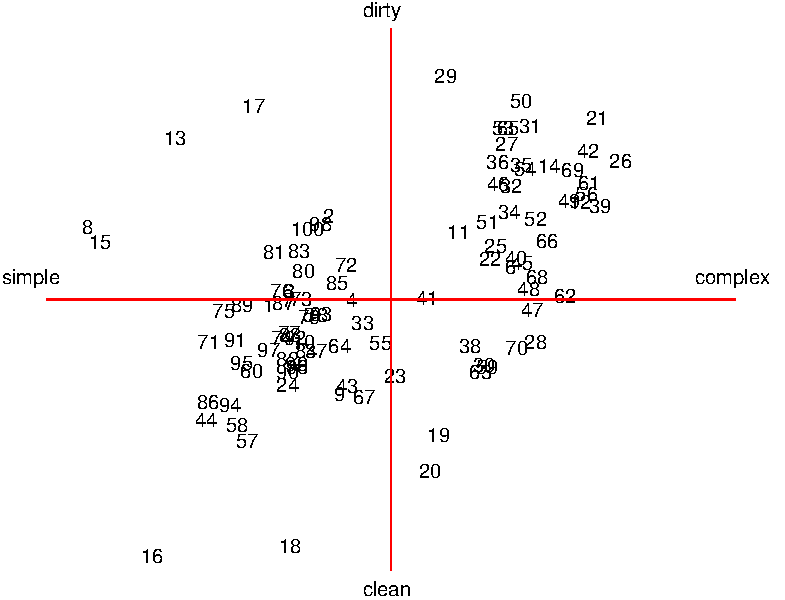
\includegraphics[width = 0.75\textwidth]{jokes_2d_2.pdf}
\caption{Two-dimensional projection of the Jester joke dataset. The
  horizontal and vertical axes correspond to the directions of the
  first and second eigenvectors, respectively, of the completed matrix
  found by the SVT algorithm on the full Jester dataset. In Table
  \ref{joketexts} we give the most extreme jokes in each direction,
  which characterize the axes.}
\label{jokes2d}
\end{figure}

In figure~\ref{jokes2d} we find that the two principal components in
the space of jokes correspond to short, simple puns (left) versus
longer, complex jokes (right), and dirty jokes (top) versus clean
jokes (bottom). Only a few jokes are given here, but at closer
inspection these observations seem to hold true in general
\footnote{Jester dataset:
  http://www.ieor.berkeley.edu/~goldberg/jester-data/}.



\section{Conclusions}

We have presented two algorithms for matrix completion, Spectral
Matrix Completion (SMC) and Spectral Value Thresholding (SVT). We
compared these sophisticated algorithms with various baselines, namely
column mean, eigentaste, and K-nearest neighbors. The comparisons are
performed with both real and synthetic data, with varying size, rank,
and sparsity. We concluded that both SMC and SVT outperform the
baseline methods. Between SMC and SVT, SMC attains better accuracy
than SVT, but at additional computational cost. For the Jester joke
dataset, we compared NMAE (Normalized Mean Absolute Error) for
different dataset sizes ({100, 200, 1000} user) on SMC, SVT,
Eigentaste, and K-nearest neighbor (with $K=50$). Spectral Matrix
Completion, an algorithm that directly minimizes the reconstruction
error, unsurprisingly leads to the best NMAE performance. In terms of
NMAE, SMC is followed by SVT, then Eigentaste, and lastly, K-nearest
neighbor. This trend follows the intuition as well.

Lastly, we presented a qualitative analysis of the low-rank assumption
central to all of our matrix completion methods. We project the 100
jokes from the Jester dataset into a two-dimensional plane and based
on the top two eigenvectors learned by the SVT algorithm. We examine
the organization of jokes in this space, and assign meaningful labels
to the axes learned by our methods. We find that the low-rank
assumption does in fact hold true for the Jester Dataset, as most of
the dimensionality is explained by the first two eigenvectors.

\begin{table} [h]
  \caption{Selection of jokes from the Jester dataset corresponding to
    the extremes of the two principal eigenvalues found by SVT. For space reasons, we omit the full text of most jokes.}
\begin{tabular}{c | l}
\hline \hline
Joke \# & Joke Text \\ \hline
  8     & Q. Did you hear about the dyslexic devil worshiper? \\
(simple)& A. He sold his soul to Santa.\\ \hline
  26 & A guy walks into a bar and sits down next to an extremely
       gorgeous woman. The first \\
(complex)& thing he notices about her though, are her pants. They were
       skin-tight, high-waisted \\
     & and had no obvious mechanism (zipper, buttons or velcro) for opening them. \\
     & After several minutes of puzzling over how she got the pants up over
       her hips, he finally \\
     & worked up the nerve to ask her. ``Excuse me miss, but how do you get into your pants?'' \\ 
     & ``Well,'' she replied, ``you can start by buying me a drink.''\\ \hline
  18 & A dog walks into Western Union and asks the clerk to send a
       telegram. He fills out a \\
(clean)& form on which he writes down the telegram he wishes to send:
       ``Bow wow wow, \\
     &  Bow wow wow.'' \\
     & The clerk says, ``You can add another 'Bow wow' for the same
       price.''\\
     & The dog responded, ``Now wouldn't that sound a little silly?''\\ \hline
  29 & An old Scotsmen is sitting with a younger Scottish gentleman
       and says the \\
(dirty)&  boy. ``Ah, lad look out that window. You see that stone wall
       there, I built it \\
     & with me own bare hands, placed every stone meself. But do they
       call me MacGregor \\
     & the wall builder? No!'' \\
     & He Takes a few sips of his beer then says, ``Aye, and look out
       on that lake and \\
     & eye that beautiful pier. I built it myself, laid every board
       and hammered each nail \\
     & but do they call me MacGregor the pier builder? No!'' \\
     & He continues...``And lad, you see that road? That too I build with me
       own bare hands. \\
     & Laid every inch of pavement meself, but do they
       call MacGregor the road builder? No!''\\
     & Again he returns to his beer for a few sips, then says,
       `` Agh, but you screw  one sheep...''\\
\hline \hline
\end{tabular}
\label{joketexts}
\end{table}
\FloatBarrier


\section{Group Member's Accomplishments}

All team members participated in all aspects of the project as well as
the final report. However, each member was responsible for taking the
lead on specific tasks. All team members contributed towards the
literature review as well. Sriram implemented Eigentaste and K-nearest
neighbor. He also had a leading role in the comparison of the methods
on the Jester dataset. Nitin and Jeeheh lead the implementation of the
SMC algorithm. Jeeheh took charge of the performance comparison on
synthetic data. Nitin got the performance metric for different
algorithms and also carried out integration of the final report.
Jonathan was in command of implementing the SVT algorithm and the two
dimensional visualizations of the Jester dataset. He also contributed
in comparing various algorithms for the synthetic dataset.


\newpage


\bibliographystyle{plain}
\bibliography{writeup}


\end{document}